\section{Problem No.1} \label{sec:prob2}
\subsection{Problem Description:} 

Consider 
$$
u_{t} =0.1 \Delta u \; \; on \; \;  \Omega = (0,1) \times (0,1)\\
\frac{\partial u}{\partial \overrightarrow{n}} = 0 \; \; on  \; \; \partial \Omega \\
u(x,y,0) = exp(-10((x-0.3)^2 +(y-0.4)^2))
$$
Write a program to solve this PDE using the Peaceman-Rachford ADI scheme on a cell-centered grid. Use a direct solver for the tridiagonal systems. In a cell-centered discretization the solution is stored at the grid points $(x_{i},y_{i}) = (\Delta x(i-0.5), \Delta x(j-0.5))$ for $i,j=1...N$ and $dx=\frac{1}{N}$. This discretization is natural for handling Neumann boundary conditions, and it is often used to discretize conservation laws. At the grid points adjacent to the boundary, the one-dimensional discrete Laplacian for homogeneous Neumann boundary conditions is 
$$
u_{xx}(x_{1}) \approx \frac{-u_{1}+u_{2}}{\Delta x^{2}}
$$
\begin{enumerate}
\item Perform a refinement study to show that your numerical solution is second-order accurate is space and time (refine time and space simultaneously using $\Delta t \propto \Delta x$) at time $t=1$.
\item Time your code for different grid sizes. Show how the computational time scales with the gird size. Compare your timing results with those from the previous homework assignment for \cn. If you had error in your codes from HW2, fix them.

Note, many of you are using script languages (MATLAB and python), and loops in these languages can be slow. You can program a single time step of ADI (in 2D) without any loops. For example, you can solve $LU=F$, where $U$ and $F$ are stored as arrays rather than vectors, and $L$ is the 1D operator to invert. Avoiding loops is not necessary for this assignment. Write your code for correctness and clarity first, and efficiency later if you have time.
\item Show that the spatial integral of the solution of the PDE does not change in time. That is 

$$
\frac{d}{dt} \int_{\Omega} u dV=0
$$
\item Show that the solution to the discrete equations satisfies the discrete conservation property 
$$
\sum_{i,j} u_{i,j}^{n} = \sum_{i,j}u_{i,j}^{0}
$$
for all $n$. Demonstrate this property with your code. 


\end{enumerate}

\subsection{Solution:} 
\paragraph{Part 1:}
The two steps ADI scheme involves decoupling of the spatial  discretization such that only one spatial direction discretization (x-sweep) is performed and advances to intermediate time step followed by the opposite spatial direction (y-sweep)and advances to the next time step. The system produces a tri-diagonal system of equation to be solved at each sweep step. The equation can be expressed under this scheme as:
$$
\frac{U_{i,j}^{n+\frac{1}{2}} - U_{i,j}^{n}}{\frac{\Delta t}{2}} = 0.1 (\frac{U_{i+1,j}^{n+\frac{1}{2}} -2U_{i,j}^{n+\frac{1}{2}} +U_{i-1,j}^{n+\frac{1}{2}}}{(\Delta x)^2} + \frac{U_{i,j+1}^{n}-2U_{i,j}^{n}+U_{i,j-1}^{n}}{(\Delta y)^2}) \;\;\;\;\;\;\;\;\; (1a)
\\
\frac{U_{i,j}^{n+1} - U_{i,j}^{n+\frac{1}{2}}}{\frac{\Delta t}{2}} = 0.1 (\frac{U_{i+1,j}^{n+\frac{1}{2}} -2U_{i,j}^{n+\frac{1}{2}} + U_{i-1,j}^{n+\frac{1}{2}}}{(\Delta x)^2} + \frac{U_{i,j+1}^{n+1}-2U_{i,j}^{n+1}+U_{i,j-1}^{n+1}}{(\Delta y)^2}) \;\;\;\;\; (1b)
$$
where equation (1a) represents the x-sweep and (1b) represents the y-sweep. After rearranging the equations, we obtain
$$
(1+2r)U_{i,j}^{n+\frac{1}{2}} - rU_{i-1,j}^{n+\frac{1}{2}} - rU_{i+1,j}^{n+\frac{1}{2}} =
(1-2r)U_{i,j}^{n}  + rU_{i,j-1}^{n}+ rU_{i,j+1}^{n} \;\;\;\;\;\;\;(2a) 
\\
(1+2r)U_{i,j}^{n+1} - rU_{i,j-1}^{n+1} - rU_{i,j+1}^{n+1} =
(1-2r)U_{i,j}^{n+\frac{1}{2}} + rU_{i-1,j}^{n+\frac{1}{2}} + rU_{i+1,j}^{n+\frac{1}{2}} \;\;\;\;\; (2b) 
$$
where $r=\frac{0.1\Delta t}{2h^2}$ and $h=\Delta x= \Delta y$. Equation (2) is used for the internal grid points. For the grid points adjacent to the boundary, we use $u_{xx}(x_{1}) \approx \frac{-u_{1}+u_{2}}{\Delta x^{2}}$ which can be derived by adding virtual points extends outside the physical domain and have values equal to the (numerical domain) boundary points. The equation can be discretized to
$$
\frac{U_{i,j}^{n+\frac{1}{2}}-U_{i,j}^{n}}{\frac{\Delta t}{2}} = 0.1(\frac{U_{i+1,j}^{n+\frac{1}{2}} - U_{i,j}^{n+\frac{1}{2}}}{h^{2}} + \frac{U_{i,j+1}^{n}-U_{i,j}^{n}}{h^{2}} )
\\
\frac{U_{i,j}^{n+1}-U_{i,j}^{n+\frac{1}{2}}}{\frac{\Delta t}{2}} = 0.1(\frac{U_{i,j+1}^{n+1} - U_{i,j}^{n+1}}{h^{2}} + \frac{U_{i+1,j}^{n+\frac{1}{2}} - U_{i,j}^{n+\frac{1}{2}}}{h^{2}} )
$$
After rearranging, the equation becomes 
$$
(1+r)U_{i,j}^{n+\frac{1}{2}} - rU_{i+1,j}^{n+\frac{1}{2}} = (1-r)U_{i,j}^{n} +rU_{i,j+1}^{n} \;\;\;\;\;\;\;\;(3a) 
\\
(1+r)U_{i,j}^{n+1} - rU_{i,j+1}^{n+1} = (1-r)U_{i,j}^{n+\frac{1}{2}} +rU_{i+1,j}^{n+\frac{1}{2}} \;\;\;\;\;\;(3b) 
$$
Since we are using cell-centered grid, the numerical solution extends from $\frac{h}{2}$ to $1-\frac{h}{2}$ in both $x$ and $y$ directions, where the physical domain extends from $[0,1]$. Thus, the smaller $h$, the closer the numerical domain gets closer to the physical domain. The expanded form of equations (2) and (3) and matrix formulation can be found in Appendix. The matrix formulation suggests that a tridiagonal system will be solved $ny$ times for the x-sweep and $nx$ times for y-sweep. The solution at different time steps on a grid of size $64 \times 64$ is shown in Figure \ref{fig:sol}.

\begin{figure}[tbh]
 \centering  
   \subfloat [time=0.0  ]{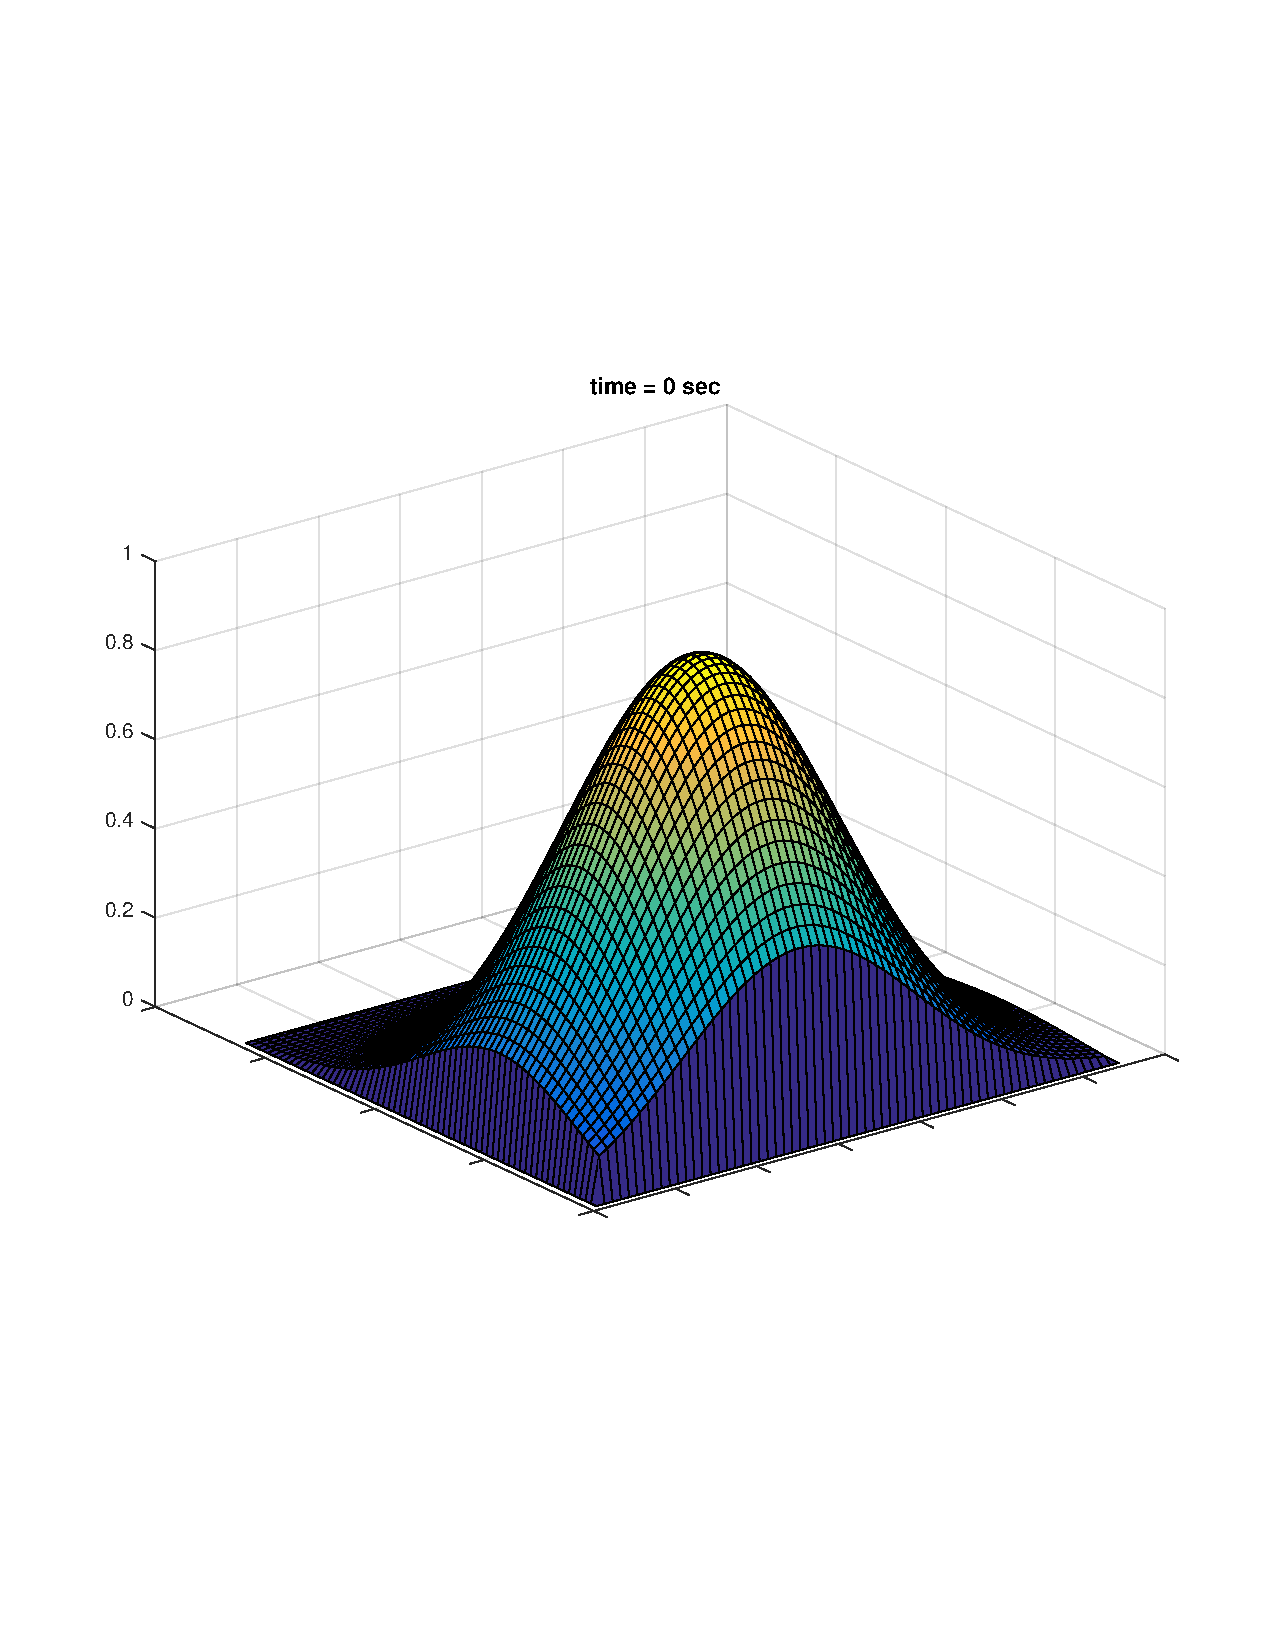
\includegraphics[scale=0.23]{fig/p1/time_0_surf.pdf}}
   \subfloat [time=0.39 ]{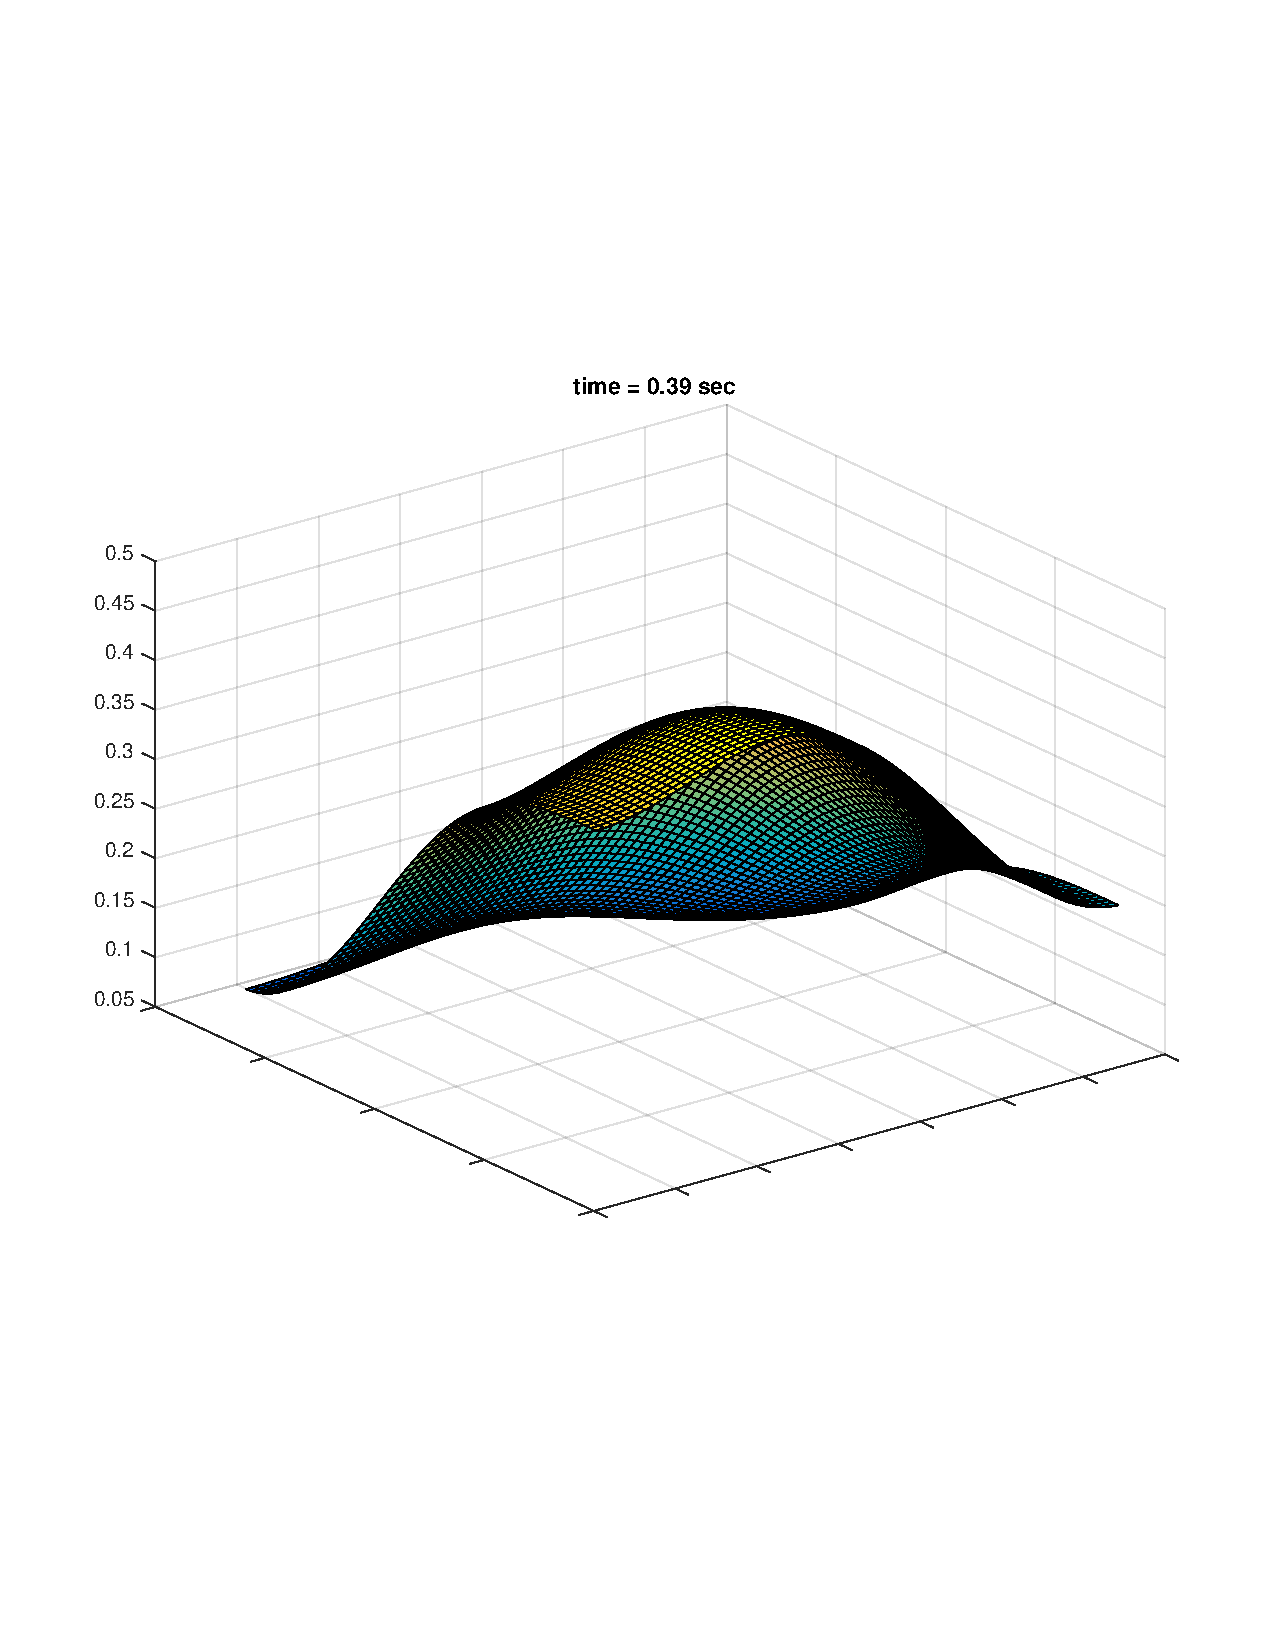
\includegraphics[scale=0.23]{fig/p1/time_0p390625_surf.pdf}}
   \subfloat [time=0.7  ]{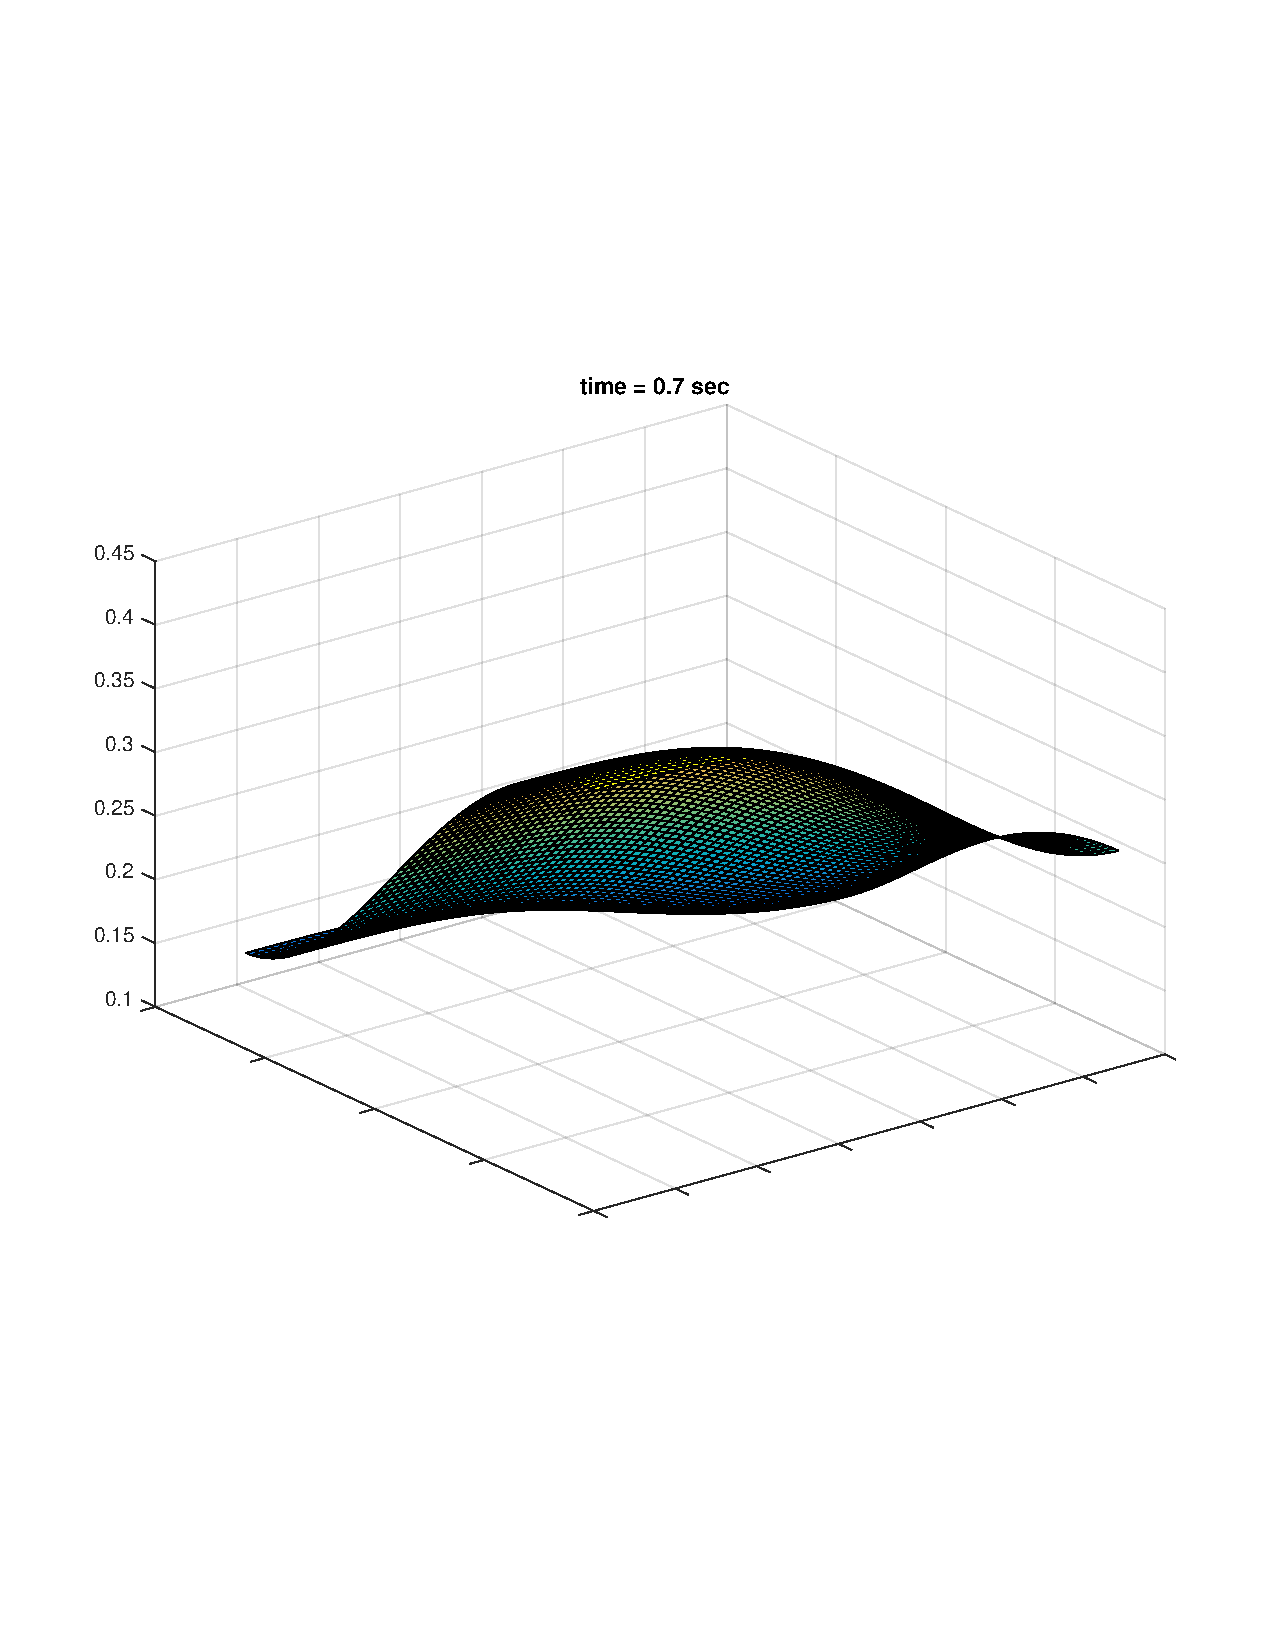
\includegraphics[scale=0.23]{fig/p1/time_0p703125_surf.pdf}}
   \subfloat [time=1.0  ]{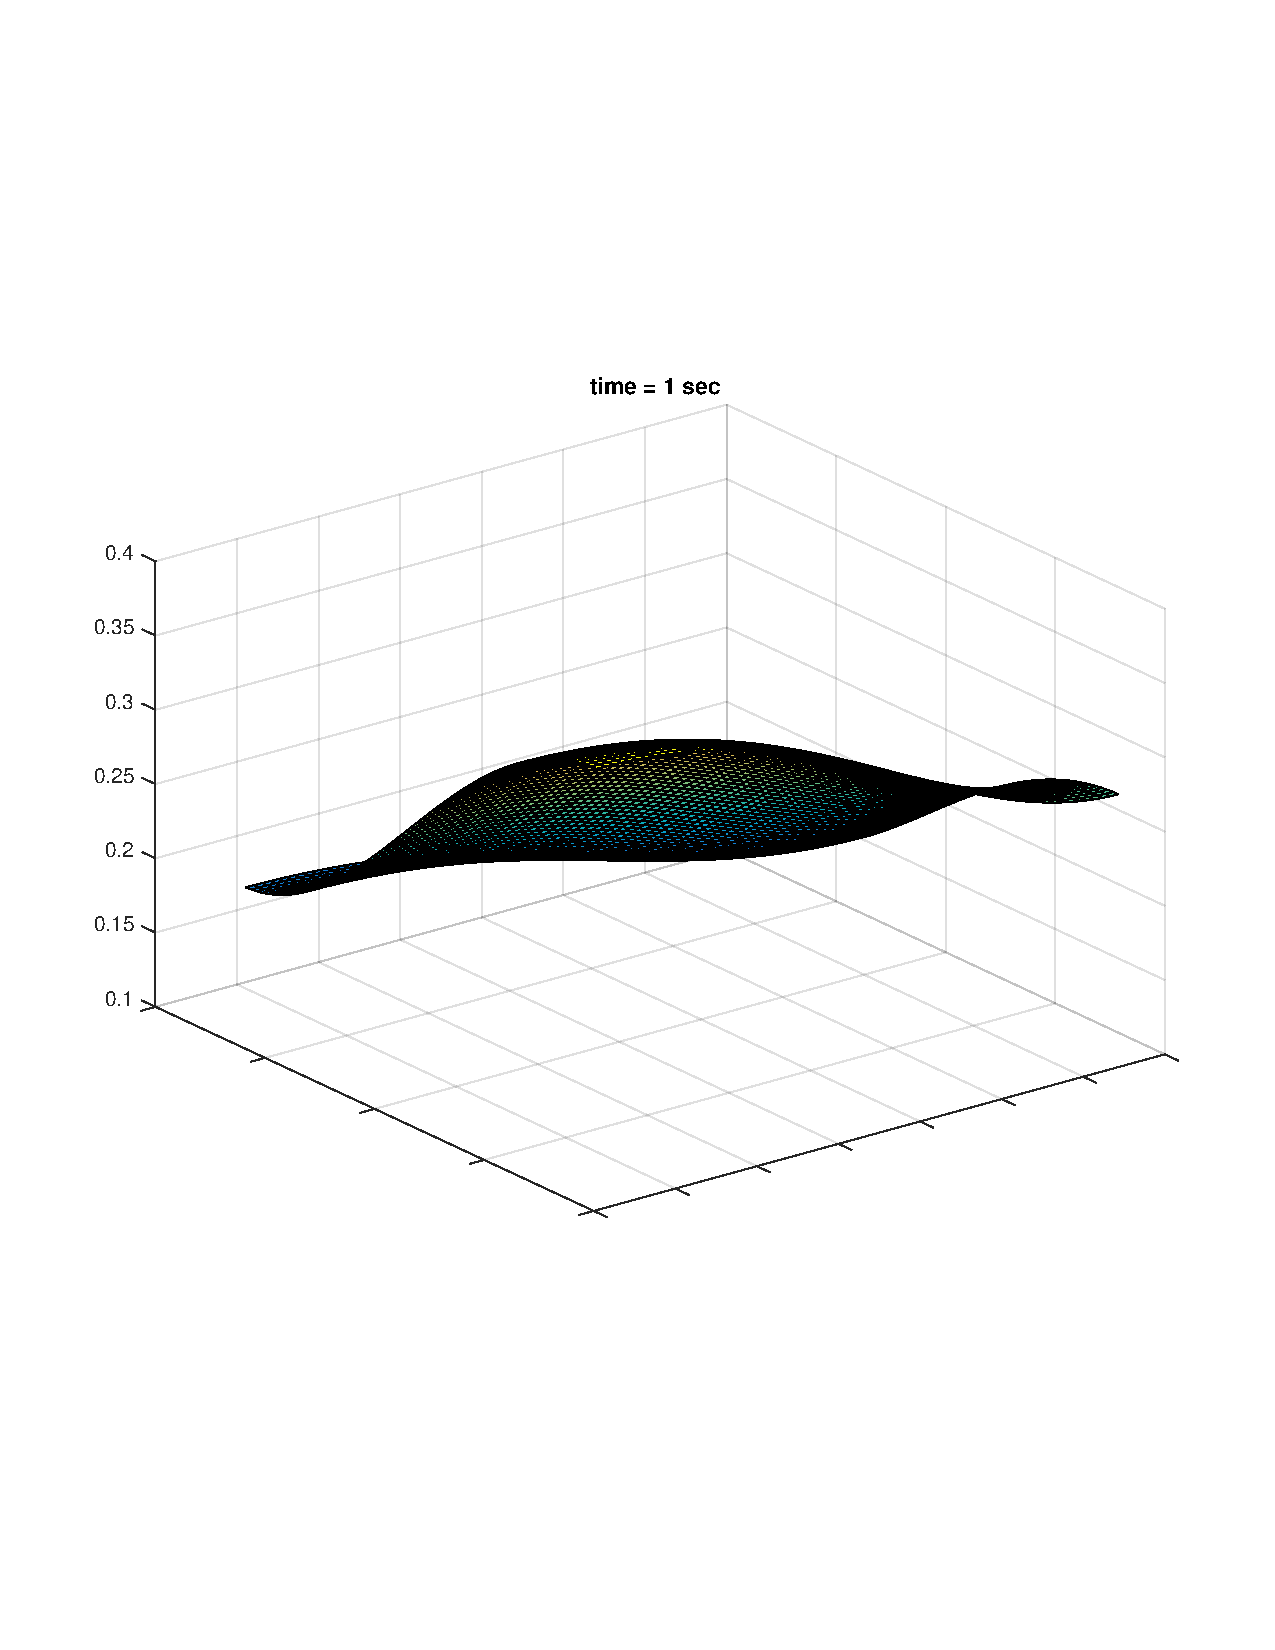
\includegraphics[scale=0.23]{fig/p1/time_1_surf.pdf}}
  \caption{The solution of problem 1 on a gird of size $64\times 64$ and time step $\Delta t = 0.001562$ as the time advances. }
   \label{fig:sol}
\end{figure} 

\paragraph{Refinement Study:} we used a similar approach as in homework 1 to carry on the refinement study. We start we certain time and space steps and calculate the sum of the solution all over the grid points. Next, we halve the time and space steps and get the sum. We then calculate the error as the absolute difference between the normalized sum of two successive solution. We then plot the total number of gird points Vs. the error on a log-log scale as shown in Figure \ref{fig:ref}(a). The slope of the line is $\approx 2.0$ which indicates that the scheme is second order accurate in space and time. 
	
\begin{figure}[tbh]
 \centering  
   \subfloat [Refinement Study]{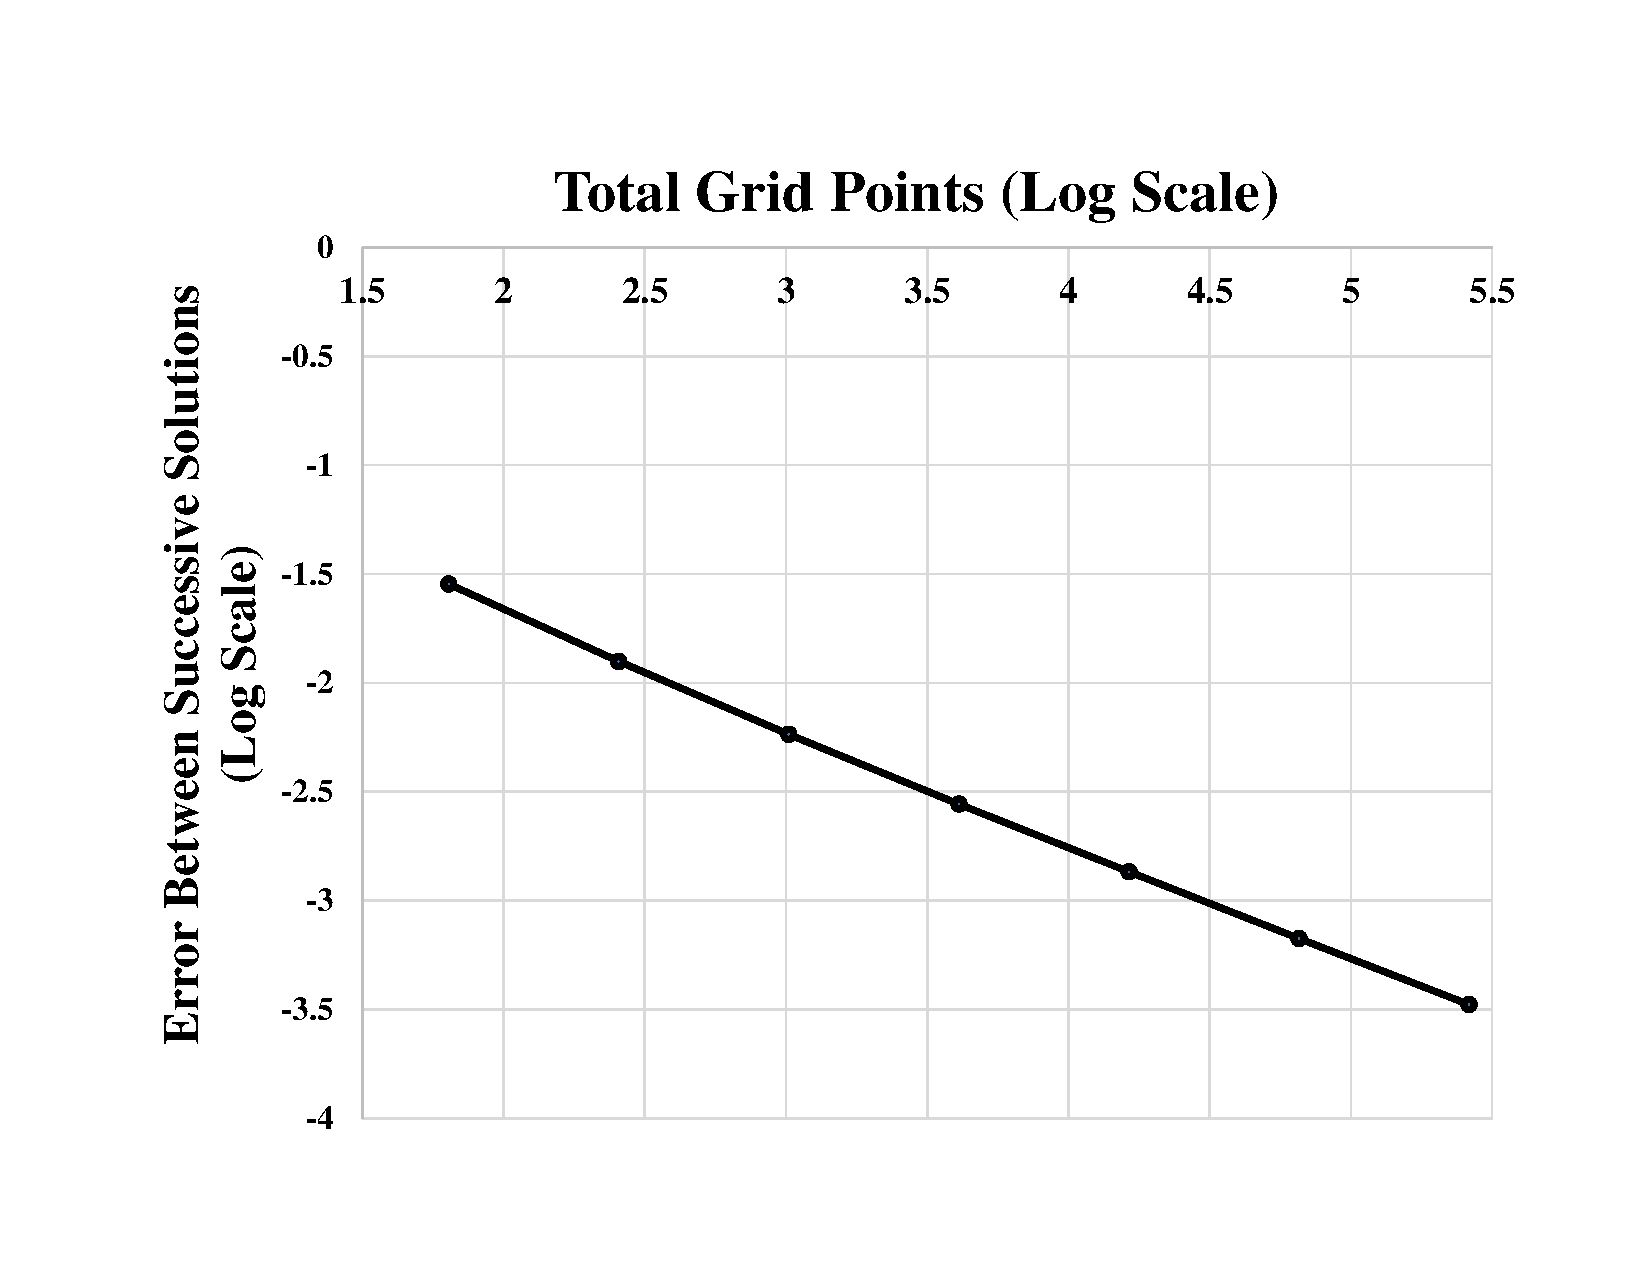
\includegraphics[width=0.4\linewidth]{fig/p1/ref.pdf}}
   \subfloat [Timing Comparison]{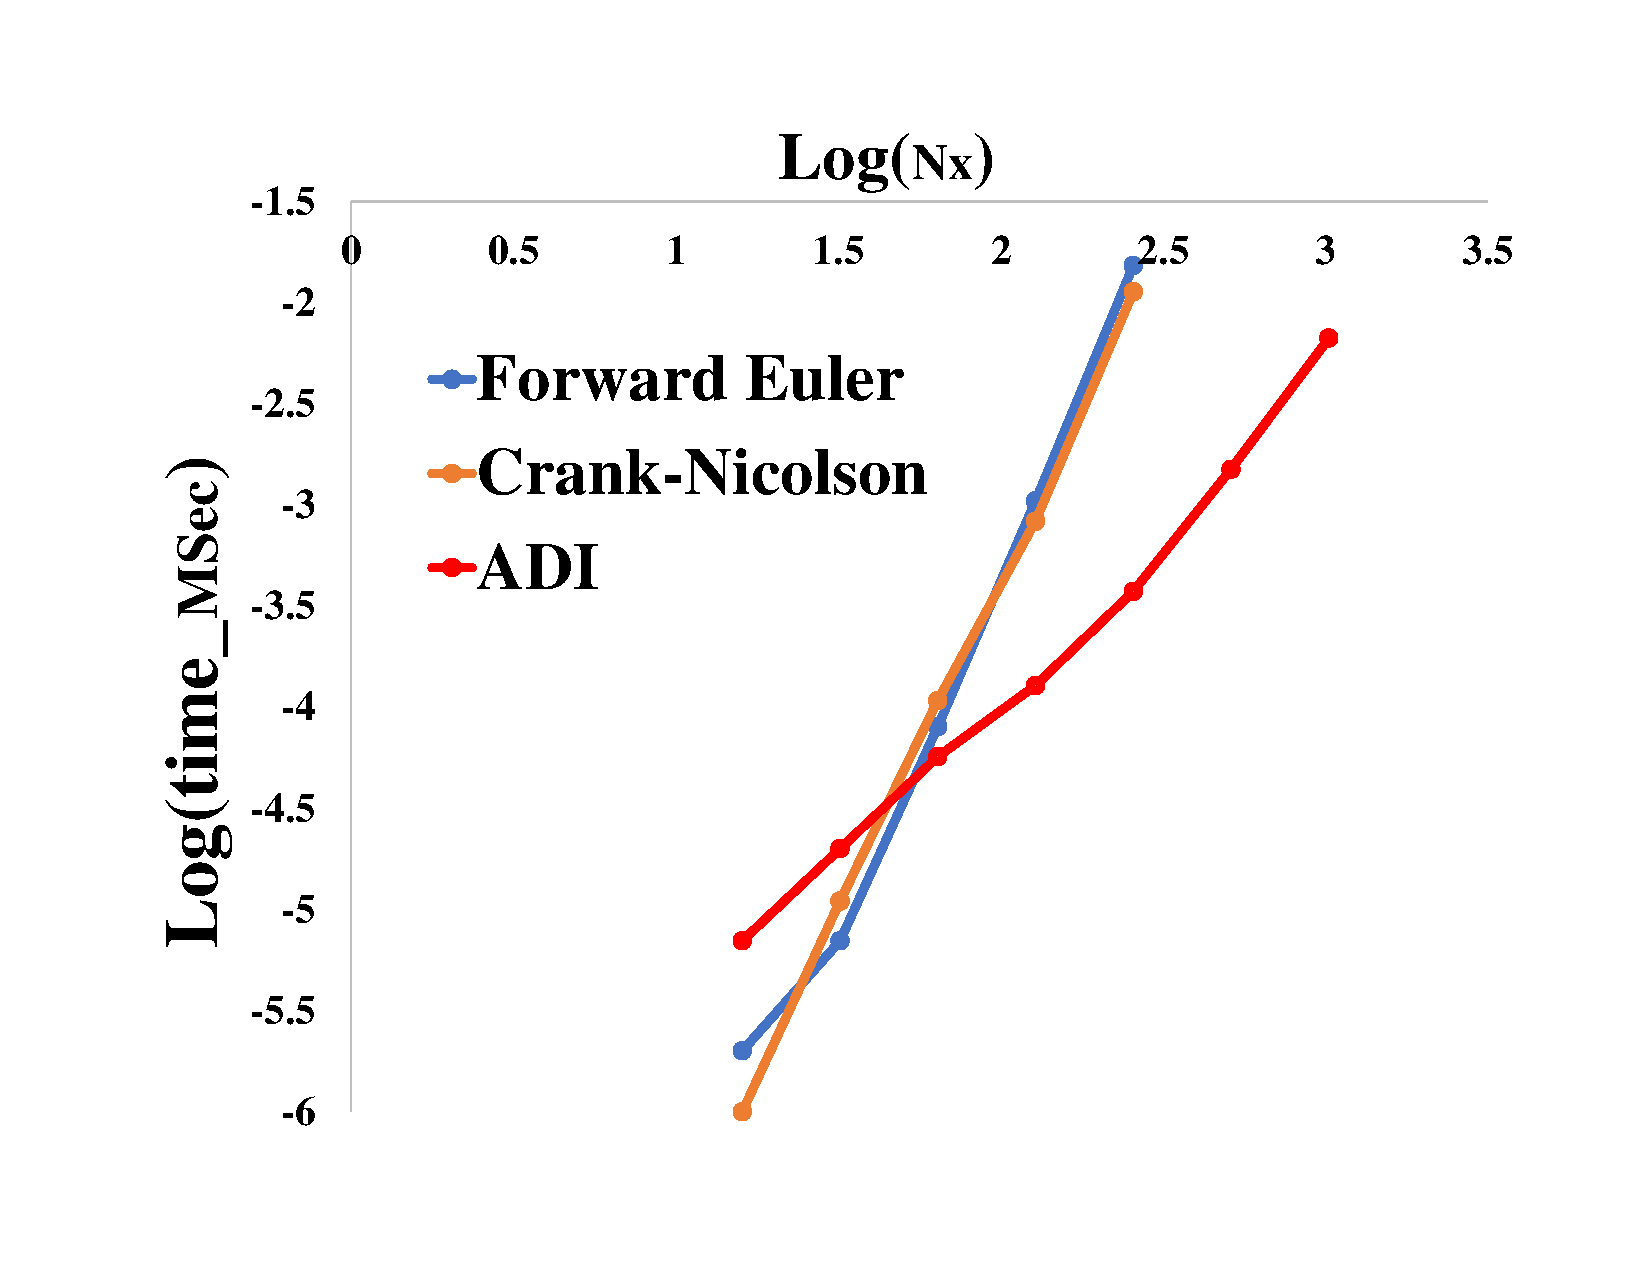
\includegraphics[width=0.4\linewidth]{fig/p1/timing.pdf}}
  \caption{Refinement study (left) shows that ADI is second order accurate in time and space. Timing comparison (right) shows the order of computational time scale for ADI, CN and Forward Euler.}
   \label{fig:ref}
\end{figure} 

\paragraph{Part 2:}
We performed a comparison between the ADI, \protect{\cn} and Forward Euler where time spacing is fixed to 0.01. The results are shown in Figure \ref{fig:ref}(b) on a log-log scale between $\Delta x$ and time in milliseconds. It is found that for small gird size, using \protect{\cn} is more efficient. But after a certain limit ($\approx 64 \times 64$ grid points), ADI becomes more superior. This is due to the fact that ADI solve a tridiagonal system which is faster to solve than the banded matrix solver for \protect{\cn}, specially that the traditional matrix solver was optimized to take in constants (not array in C++) since the value of a single diagonal are the same. 


\paragraph{Part 3:}
This part asks to prove that the concentration will not change with time which is implied due to the insulated boundary (following the conservation of mass), or $\frac{d}{dt} \int_{\Omega} u.dV=0$. We can change the order of differentiation and integration and since $u_{t}=0.1\Delta u$, then we get
$$
\frac{d}{dt} \int_{\Omega} u.dV= \int_{\Omega} \frac{d u}{dt}.dV  = \int_{\Omega} 0.1\Delta u.dV
$$
Since $u$  is function in $x$ and $y$ and each extends from 0 to 1:
$$
\frac{d}{dt} \int_{\Omega} u.dV =  0.1 \int_{0}^{1}\int_{0}^{1}\frac{\partial^{2}u}{\partial x^{2}} + \frac{\partial^{2}u}{\partial y^{2}}.dxdy  = 0.1 (\int_{0}^{1}\int_{0}^{1}\frac{\partial^{2}u}{\partial x^{2}}.dxdy + \int_{0}^{1}\int_{0}^{1}\frac{\partial^{2}u}{\partial y^{2}} .dydx)
$$

Using the fundamental theorem of calculus to obtain solution for single integration, we get 
$$
\int_{0}^{1}\frac{\partial^{2}u}{\partial x^{2}}.dx = \frac{\partial u^2}{\partial x^2}|_{x=1} - \frac{\partial u^2}{\partial x^2}|_{x=0}
$$
The boundary conditions suggest that there no material crossing the boundary and thus $\frac{\partial u}{\partial x}=0$ along the boundary ($x=0$ and $x=1$). Thus 
$$
\int_{0}^{1}\frac{\partial^{2}u}{\partial x^{2}}.dx = 0
$$
Similarly, we can prove that
$$
\int_{0}^{1}\frac{\partial^{2}u}{\partial y^{2}}.dy = 0
$$
Plugging these results back to the original equation, we get
$$
\frac{d}{dt} \int_{\Omega} u.dV =  0.1 \int_{0}^{1}\int_{0}^{1}\frac{\partial^{2}u}{\partial x^{2}} + \frac{\partial^{2}u}{\partial y^{2}}.dxdy = 0
$$

\paragraph{Part 4:}
For this part, if we prove that the summation equals for two time steps $t=n$ and $t=n+1$, then it is proven for the time steps $t=0$ and $t=n$ (by the virtue that the summation for all intermediate time steps between $t=0$ and $t=n$ are the same). We start by writing the first couple of equations for the x-sweep which will give us the summation $\sum_{i,j}U_{i,j}^{n}$. Here we use small and capital $u$ interchangeable.

$$
i=0, j=0 \rightarrow (1+r)U_{0,0}^{n+\frac{1}{2}} - rU_{1,0}^{n+\frac{1}{2}} = (1-r)U_{0,0}^{n}+rU_{0,1}^{n}
\\
i=1, j=0 \rightarrow (1+2r)U_{1,0}^{n+\frac{1}{2}} - rU_{0,0}^{n+\frac{1}{2}} - rU_{2,0}^{n+\frac{1}{2}} = (1-r)U_{1,0}^{n} + rU_{1,1}^{n}
\\
i=2, j=0 \rightarrow (1+2r)U_{2,0}^{n+\frac{1}{2}} - rU_{1,0}^{n+\frac{1}{2}} - rU_{3,0}^{n+\frac{1}{2}} = (1-r)U_{2,0}^{n} + rU_{2,1}^{n}
\\
............
\\
..........
\\
i=0, j=1 \rightarrow (1+r)U_{0,1}^{n+\frac{1}{2}} - rU_{1,1}^{n+\frac{1}{2}} = (1-2r)U_{0,1}^{n}+rU_{0,0}^{n}+rU_{0,2}^{n}
\\
i=1, j=1 \rightarrow (1+2r)U_{1,1}^{n+\frac{1}{2}} - rU_{0,1}^{n+\frac{1}{2}} - rU_{2,1}^{n+\frac{1}{2}} = (1-2r)U_{1,1}^{n}+ rU_{1,0}^{n} + rU_{1,2}^{n}
\\
i=2, j=1 \rightarrow (1+2r)U_{2,1}^{n+\frac{1}{2}} - rU_{1,1}^{n+\frac{1}{2}} - rU_{3,1}^{n+\frac{1}{2}} = (1-2r)U_{2,1}^{n} + rU_{2,0}^{n}+ rU_{2,2}^{n}
\\
.............
\\
..........
\\
i=0, j=2 \rightarrow (1+r)U_{0,2}^{n+\frac{1}{2}} - rU_{1,2}^{n+\frac{1}{2}} = (1-2r)U_{0,2}^{n}+rU_{0,1}^{n} + rU_{0,3}^{n}
\\
i=1, j=2 \rightarrow (1+2r)U_{1,2}^{n+\frac{1}{2}} - rU_{0,2}^{n+\frac{1}{2}} - rU_{2,2}^{n+\frac{1}{2}} = (1-2r)U_{1,2}^{n}+ rU_{1,1}^{n} + rU_{1,3}^{n}
\\
i=2, j=2 \rightarrow (1+2r)U_{2,2}^{n+\frac{1}{2}} - rU_{1,2}^{n+\frac{1}{2}} - rU_{3,2}^{n+\frac{1}{2}} = (1-2r)U_{2,2}^{n} + rU_{2,1}^{n}+ rU_{2,3}^{n}
\\
.............
\\
..........
$$
Now we sum, the right hand side will give 

$$
U_{0,0}^{n} + U_{0,1}^{n} + U_{0,2}^{n}+ ..........
U_{1,0}^{n} + U_{1,1}^{n} + U_{1,2}^{n}+ ..........
U_{2,0}^{n} + U_{2,1}^{n} + U_{2,2}^{n}+ .......... = \sum	_{i,j}U_{i,j}^{n}
$$
Summing the left hand side gives
$$
U_{0,0}^{n+\frac{1}{2}} + U_{0,1}^{n+\frac{1}{2}} + U_{0,2}^{n+\frac{1}{2}}+ ..........
U_{1,0}^{n+\frac{1}{2}} + U_{1,1}^{n+\frac{1}{2}} + U_{1,2}^{n+\frac{1}{2}}+ ..........
U_{2,0}^{n+\frac{1}{2}} + U_{2,1}^{n+\frac{1}{2}} + U_{2,2}^{n+\frac{1}{2}}+ .......... \\= \sum	_{i,j}U_{i,j}^{n+\frac{1}{2}}
$$
We can do the same process for the y-sweep to obtain $\sum_{i,j}U_{i,j}^{n+1}$ such that

$$
i=0, j=0 \rightarrow (1+r)U_{0,0}^{n+1} - rU_{0,1}^{n+1} = (1-r)U_{0,0}^{n+\frac{1}{2}}+rU_{1,0}^{n+\frac{1}{2}}
\\
i=0, j=1 \rightarrow (1+2r)U_{0,1}^{n+1} - rU_{0,0}^{n+1} - rU_{0,2}^{n+1} = (1-r)U_{0,1}^{n+\frac{1}{2}} + rU_{1,1}^{n+\frac{1}{2}}
\\
i=0, j=2 \rightarrow (1+2r)U_{0,2}^{n+1} - rU_{0,1}^{n+1} - rU_{0,3}^{n+1} = (1-r)U_{0,2}^{n+\frac{1}{2}} + rU_{1,2}^{n+\frac{1}{2}}
\\
............
\\
..........
\\
i=1, j=0 \rightarrow (1+r)U_{1,0}^{n+1} - rU_{1,1}^{n+1} = (1-2r)U_{1,0}^{n+\frac{1}{2}}+rU_{0,0}^{n+\frac{1}{2}}+rU_{2,0}^{n+\frac{1}{2}}
\\
i=1, j=1 \rightarrow (1+2r)U_{1,1}^{n+1} - rU_{1,0}^{n+1} - rU_{1,2}^{n+1} = (1-2r)U_{1,1}^{n+\frac{1}{2}}+ rU_{0,1}^{n+\frac{1}{2}} + rU_{2,1}^{n+\frac{1}{2}}
\\
i=1, j=2 \rightarrow (1+2r)U_{1,2}^{n+1} - rU_{1,1}^{n+1} - rU_{1,3}^{n+1} = (1-2r)U_{1,2}^{n+\frac{1}{2}} + rU_{0,2}^{n}+ rU_{2,2}^{n+\frac{1}{2}}
\\
.............
\\
..........
\\
i=2, j=0 \rightarrow (1+r)U_{2,0}^{n+1} - rU_{2,1}^{n+1} = (1-2r)U_{2,0}^{n+\frac{1}{2}}+rU_{1,0}^{n+\frac{1}{2}} + rU_{3,0}^{n+\frac{1}{2}}
\\
i=2, j=1 \rightarrow (1+2r)U_{2,1}^{n+1} - rU_{2,0}^{n+1} - rU_{2,2}^{n+1} = (1-2r)U_{2,1}^{n+\frac{1}{2}}+ rU_{1,1}^{n+\frac{1}{2}} + rU_{3,1}^{n+\frac{1}{2}}
\\
i=2, j=2 \rightarrow (1+2r)U_{2,2}^{n+1} - rU_{2,1}^{n+1} - rU_{2,3}^{n+1} = (1-2r)U_{2,2}^{n+\frac{1}{2}} + rU_{1,2}^{n+\frac{1}{2}}+ rU_{3,2}^{n+\frac{1}{2}}
\\
.............
\\
..........
$$

Summing the left hand side will give $\sum_{i,j}U_{i,j}^{n+1}$ such that
$$
U_{0,0}^{n+1} + U_{0,1}^{n+1} + U_{0,2}^{n+1}+ ..........
U_{1,0}^{n+1} + U_{1,1}^{n+1} + U_{1,2}^{n+1}+ ..........
U_{2,0}^{n+1} + U_{2,1}^{n+1} + U_{2,2}^{n+1}+ ..........\\ = \sum	_{i,j}U_{i,j}^{n+1}
$$
while the right hand side gives $\sum_{i,j}U_{i,j}^{n+\frac{1}{2}}$. Since 
$$
\sum_{i,j}U_{i,j}^{n} = \sum_{i,j}U_{i,j}^{n+\frac{1}{2}} = \sum_{i,j}U_{i,j}^{n+1}
$$
We conclude that this equality holds for $\sum_{i,j}U_{i,j}^{0} = \sum_{i,j}U_{i,j}^{n}$ as well. 

We used the code to verify the above statement by printing the summation of the solution at all gird points for different intermediate time steps (with fixed $nx$ and $ny$). The results shown in Table \ref{tab:sum} agrees with our proof. 

\begin{table*}[h!]
\centering
\begin{tabular}{|c|c|}
\hline
Time & $\sum_{i,j}U_{i,j}$  \\ 
\hline
0.0015625 & 1111.666239  \\ 
0.0031250 & 1111.666239  \\  
0.0046875 & 1111.666239  \\
0.00625 & 1111.666239  \\
0.0078125 & 1111.666239  \\
0.009375& 1111.666239  \\
0.0109375 & 1111.666239  \\
 0.0140625 & 1111.666239  \\
 0.015625 & 1111.666239  \\
0.0171875 & 1111.666239  \\
..... & ....  \\
..... & ....  \\
..... & ....  \\
0.996875 & 1111.666239  \\
0.9984375 & 1111.666239  \\
 1 & 1111.666239  \\
\end{tabular}
\caption{Summing the solution over all grid points for different time steps (fixed $nx$ and $ny$)}
\label{tab:sum}
\end{table*}